\newpage
{\bfseries IRSTI 50.47.29}

\sectionwithauthors{U. Imanbekova, A. Kalizhanova, A.Kozbakova, A. Imanbekova, A.Utegenova}{DEVELOPMENT OF AN ALGORITHM FOR ADAPTING A MATHEMATICAL MODEL OF THE PROCESS OF MIXING AND MELTING COPPER CONCENTRATES}

\begin{center}
{\bfseries U. Imanbekova\textsuperscript{1}, A.
Kalizhanova\textsuperscript{2,1}, A.Kozbakova\textsuperscript{2,3}, A.
Imanbekova\textsuperscript{4}, A.Utegenova\textsuperscript{1,2}}

\textsuperscript{1}Almaty University of Power Engineering and
Telecommunications named after G.Daukeyev, Almaty, Kazakhstan,

\textsuperscript{2}Institute of Information and Computational
Technologies CS MSHE RK, Almaty, Kazakhstan,

\textsuperscript{3}Almaty Technological University, Almaty, Kazakhstan,

\textsuperscript{4}Taraz Regional University named after M.Kh. Dulaty,
Taraz, Kazakhstan,

е-mail: uli.08@mail.ru
\end{center}

The paper describes the information base of the system, which is formed
by algorithms of centralized control, automated analytical control
system and control data of material flows. The data processing algorithm
according to a special program generates additional information
necessary to solve the control tasks of the system and includes
algorithms for processing analytical data information, as well as data
for monitoring material flows, calculations of additional electric
furnace variables, loading of charge into furnace bunkers and
technological variables by department. The simulation model of the
functioning of the complex "technological process -- control system" is
implemented in the form of a package of interconnected software modules.
The package implementing the simulation model is divided into three
complexes: a set of programs for "Data collection and processing"; a
complex for "Optimal process control"; a set of programs for "optimal
energy regime management".

{\bfseries Keywords.} Copper raw materials, blending, smelting,
mathematical model, mixing and melting.

\begin{center}
{\large\bfseries МЫС КОНЦЕНТРАТТАРЫН АРАЛАСТЫРУ ЖӘНЕ БАЛҚЫТУ ПРОЦЕСІ ҮШІН
МАТЕМАТИКАЛЫҚ МОДЕЛЬДІ БЕЙІМДЕУ АЛГОРИТМІН ӘЗІРЛЕУ}

{\bfseries У.Иманбекова\textsuperscript{1},А.Калижанова\textsuperscript{2,1},
А.Козбакова\textsuperscript{2,3}, А.Иманбекова\textsuperscript{4},
А.Утегенова\textsuperscript{1,2}}

\textsuperscript{1}Ғ.Дәукеев атындағы Алматы энергетика және байланыс
университеті, Алматы, Қазақстан,

\textsuperscript{2}Ақпараттық және есептеуіш технологиялар институты ҚР
ҒЖБМ ҒК, Алматы, Қазақстан,

\textsuperscript{3}Алматы технологиялық университеті, Алматы, Қазақстан,

\textsuperscript{4}М.Х. Дулати атындағы Тараз өңірлік университеті,
Тараз, Қазақстан,

е-mail: uli.08@mail.ru
\end{center}

Мақалада орталықтандырылған басқару алгоритмдерімен, аналитикалық
бақылаудың автоматтандырылған жүйесімен және материалдық Ағындарды
бақылау деректерімен қалыптасатын жүйенің ақпараттық базасы сипатталған.
Арнайы бағдарлама бойынша деректерді өңдеу алгоритмі жүйені басқару
мәселелерін шешу үшін қажетті қосымша ақпаратты жасайды және
аналитикалық ақпаратты өңдеу алгоритмдерін, сондай-ақ материалдық
Ағындарды бақылау, электр пешінің қосымша параметрлерін есептеу, пештің
бункерлеріне шихтаны жүктеу және цехтар бойынша технологиялық
параметрлерді қамтиды. «Технологиялық процесс -- басқару жүйесі»
кешенінің жұмыс істеуінің имитациялық моделі өзара байланысты
бағдарламалық модульдер пакеті түрінде іске асырылды. Модельдеу моделін
жүзеге асыратын Пакет үш кешенге бөлінеді: «деректерді жинауға және
өңдеуге» арналған бағдарламалар жиынтығы; «технологиялық процесті
оңтайлы басқаруға» арналған кешен; «оңтайлы энергетикалық режимді
басқаруға» арналған бағдарламалар жиынтығы.

{\bfseries Түйін сөздер:} мыс шикізаты, араластыру, балқыту, математикалық
модель, араластыру және балқыту.

\begin{center}
{\large\bfseries РАЗРАБОТКА АЛГОРИТМА АДАПТАЦИИ МАТЕМАТИЧЕСКОЙ МОДЕЛИ ДЛЯ
ПРОЦЕССА СМЕШИВАНИЯ И ПЛАВЛЕНИЯ МЕДНЫХ КОНЦЕНТРАТОВ}

{\bfseries У.Иманбекова\textsuperscript{1},А.Калижанова\textsuperscript{2,1},
А.Козбакова\textsuperscript{2,3}, А.Иманбекова\textsuperscript{4},
А.Утегенова\textsuperscript{1,2}}

\textsuperscript{1}Алматинский университет энергетики и связи им. Г.
Даукеева, Алматы, Казахстан.

\textsuperscript{2}Институт информационных и вычислительных технологий
КН МНВО РК, Алматы, Казахстан,

\textsuperscript{3}Алматинский технологический университет, Алматы,
Казахстан,

\textsuperscript{4}Таразский региональный университет им.М. Х. Дулати,
Тараз, Казахстан,

е-mail: uli.08@mail.ru
\end{center}

В статье описана информационная база системы, которая формируется
алгоритмами централизованного управления, автоматизированной системой
аналитического контроля и данными контроля материальных потоков.
Алгоритм обработки данных по специальной программе генерирует
дополнительную информацию, необходимую для решения задач управления
системой, и включает в себя алгоритмы обработки аналитической
информации, а также данные для мониторинга материальных потоков,
расчетов дополнительных параметров электропечи, загрузки шихты в бункеры
печи и технологических параметров по цехам. Имитационная модель
функционирования комплекса "технологический процесс -- система
управления" реализована в виде пакета взаимосвязанных программных
модулей. Пакет, реализующий имитационную модель, разделен на три
комплекса: набор программ для "Сбора и обработки данных"; комплекс для
"Оптимального управления технологическим процессом"; набор программ для
"управления оптимальным энергетическим режимом".

{\bfseries Ключевые слова.} Медное сырье, смешивание, плавка,
математическая модель, смешивание и плавка.

\begin{multicols}{2}
{\bfseries Introduction.} To predict process variables using an adaptive
mathematical model, constant updated samples containing a certain number
of observations of the process must be stored in the PC memory {[}1{]}.
When the operator enters the code of a certain equation of the model,
the corresponding values of the model parameters, object variables and
algorithm constants are received at the algorithm input, the adjusted
model parameters and the predicted value of the object variable are
printed {[}2{]}.

The analytical information processing algorithm generates information
about the chemical compositions of material flows necessary for solving
functional control tasks using information arrays generated by an
automated analytical control system based on \emph{X-ray} spectral
equipment {[}3{]}. The data is sent to the computer of the automated
control system of the metallurgical workshop via interprocessor
communication channels as they are formed. The data on the chemical
composition of the melting products relate to the moments of discharge
of these products, which are random in nature {[}4{]}. The output
information of the algorithm is preprocessed information about the
chemical composition of material flows {[}5{]}.

Based on the data of the daily work schedule of the electric furnace
department, which determines the number of processed granules,
revolutions, limestone, liquid converter slag, a given electrical power,
taking into account the current chemical composition of the loaded
materials, a table of initial data was filled in, which were transmitted
via communication channels to the information and computing center
{[}6{]}. The obtained data of the optimal technological regime were
printed out and transmitted to the shift foreman in the form of a task
for implementation during the process {[}7{]}.

{\bfseries Materials and methods.} During the tests, the following values
characterizing the electric melting process were recorded in the
observation log: date and shift number, set and actual, number of loaded
materials (by type), power consumption, electric power of the furnace,
current and voltage at the electrodes, the amount of matte produced, the
amount of fused slag; the results of chemical analyses of the loaded
materials and the products received; the surname of the replacement
master; the time of solving the problem on the PC {[}8{]}.

The tests were carried out in two stages: at the first, data was
collected during the usual (existing) control of the electric welding
process, at the second -- during the implementation of the process
according to the optimal control algorithm {[}9{]}.

The choice of a working algorithm for adapting a mathematical model that
best satisfies the condition of accuracy of approximation by the model
of the output variables of an object over a time interval of length is
reduced to determining the type of operators
\(\psi\{.\},\left\{ . \right\}\) of the sequence type
\(\gamma\lbrack k\rbrack\), the value of constants \(\eta\), and the
minimum sample length {[}10{]}.

We present a working algorithm for adapting the mathematical model of
electric melting.

The adaptation algorithm calculates the current values of the parameters
of the mathematical model based on the initial data:

a) the current values of the output and input variables of the adapting
equation (model).

b) the values of the parameters obtained at the previous step of the
algorithm;

c) values of constants;

d) the calculated value of the output variable obtained at the previous
step of the algorithm.

The output information of the algorithm is the adjusted values of the
equation parameters to the following Equation 1.
\end{multicols}

\begin{equation}
\xi = \delta_{0} + \sum_{i = 1}^{m}\delta_{i}\psi_{i}
\end{equation}

Minimizing the square of the mismatch between the actual (measured at
the nth instant of time) value of the output variable to its calculated
value to the following Equation 2.

\begin{equation}
\Delta\xi = (\xi\lbrack n\rbrack - \delta_{0} - \sum_{i = 1}^{m}{\delta_{i}\psi_{i}}\lbrack n\rbrack)^{2}
\end{equation}

Where \(\xi\lbrack n\rbrack\) is the output variable of the model, Here:

\(\psi_{i}\lbrack n\rbrack,(i = \overline{1,m})\) - input variables of
the model,

n=1,2,... - discrete time,

\(\delta_{0},\delta_{i}(i = \overline{1,m})\) - equation parameters.

Calculation formulas to the following Equations 3-10:

\begin{equation}
\langle\frac{\delta_{o}\lbrack k\rbrack = \delta_{o}\lbrack k - 1\rbrack + t\lbrack k\rbrack\gamma_{o}\lbrack k\rbrack\Delta\varepsilon\lbrack n,k - 1\rbrack}{\delta_{i}\lbrack k\rbrack = \delta_{i}\lbrack k - 1\rbrack + t\lbrack k\rbrack\gamma_{i}\lbrack k\rbrack\Delta\varepsilon\lbrack n,k - 1\rbrack\psi_{i}\lbrack n\rbrack}
\end{equation}

\begin{equation}
\delta_{i}\lbrack k\rbrack = \delta_{i}\lbrack k - 1\rbrack(i = 0,1,...),
\end{equation}

\begin{equation}
\Delta\varepsilon\lbrack n,k\rbrack = \overline{\varepsilon}\lbrack n\rbrack - \breve{\varepsilon}\lbrack n,k\rbrack
\end{equation}

\begin{equation}
\breve{\varepsilon}\lbrack n,k\rbrack = \delta_{0}\lbrack k\rbrack + \sum_{i = 1}^{m}{\delta_{i}\lbrack k\overline{\rbrack\psi}\lbrack n\rbrack}
\end{equation}

\begin{equation}
\overline{\varepsilon}\lbrack n\rbrack = \overline{\varepsilon}\lbrack n - 1\rbrack + \frac{1}{T_{\varepsilon}}(\varepsilon\lbrack n\rbrack - \overline{\varepsilon}\lbrack n - 1\rbrack,\quad (i = \overline{1,m)}
\end{equation}

\begin{equation}
\overline{\varepsilon}\lbrack n\rbrack = \overline{\varepsilon}\lbrack n - 1\rbrack + \frac{1}{T_{\varepsilon}}(\varepsilon\lbrack n\rbrack - \overline{\varepsilon}\lbrack n - 1\rbrack)
\end{equation}

\begin{equation}
t\lbrack k\rbrack = 1 + r/\Delta\varepsilon\lbrack n - 1,k - 1\rbrack + \Delta\varepsilon\lbrack n - 2,k - 2\rbrack
\end{equation}

\begin{equation}
\gamma_{i}\lbrack k\rbrack = \left( \begin{aligned}
 & \overline{\gamma_{i}} = const\ if\ \eta\lbrack\gamma\rbrack = 1 \\
 & \frac{\gamma_{i}\lbrack 0\rbrack}{S\lbrack n\rbrack},if\eta\lbrack х\gamma\rbrack = 0
\end{aligned} \right.
\end{equation}

Where:

\(S\lbrack n\rbrack\) - the number of steps of the algorithm after the
next violation of the condition
\(\left. \ \Delta\varepsilon\lbrack n,k\rbrack \right| \leq \Delta\).

\(\overline{\psi}\lbrack n\rbrack,\overline{\varepsilon}\lbrack n\rbrack\)
- variables formed by sliding averaging over intervals, respectively
\(T_{i}\)и \(T_{\varepsilon}\);

\(\delta_{i}\lbrack k\rbrack,(i = \overline{0,m})\) - equation
parameters corresponding to the kth step (iteration) of the algorithm;

\(\overset{̑}{\varepsilon}\lbrack n.k\rbrack\) - calculated values of the
output variable corresponding to time n, obtained using the parameters
\(\delta_{i}\lbrack k\rbrack\);

\(\gamma_{i}\lbrack k\rbrack,(i = \overline{0,m})\) - The iteration step
is positive numbers that determine the amount of parameter correction at
the kth step of the algorithm;

\(t\lbrack k\rbrack\) - accelerating multiplier;

\(\eta\lbrack\gamma\rbrack\) - a constant that defines the type of
sequence \(\gamma_{i}\lbrack k\rbrack(k = 1,2,...)\);

\(\Delta > 0\) - the threshold value of the misalignment of the value
\(\varepsilon\lbrack n\rbrack и\widetilde{\varepsilon}\lbrack n,k\rbrack\).

{\bfseries Results and discussion.} The flowchart of the algorithm is
described in this way:

Block 1 performs the sequential formation of arrays necessary for
calculation from the total array of data.

Block 2 checks the completeness of information generation.

Block 3 checks the receipt of new analytical information.

The block diagram of the algorithm for processing analytical information
in Figure 1.

\begin{figure}[H]
	\centering
	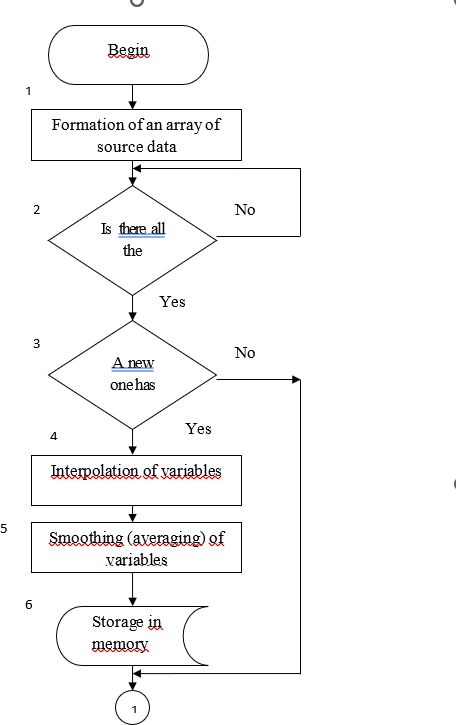
\includegraphics[width=0.4\textwidth]{assets/7}
	\caption*{Figure 1 - The block diagram of the algorithm for processing analytical information}
\end{figure}

Block 4 calculates the interpolated value of the content of the i-th
component of the j-th material of the k-th furnace to the following
Equation 11:

\begin{equation}
Χ_{ijk}\lbrack n\rbrack = Χ_{ijk_{}}\lbrack\mu\rbrack - \frac{\left( Χ_{ijk}\lbrack\mu\rbrack - Χ_{ijk}\lbrack\mu\rbrack \right)\left( n - \tau_{\mu} \right)}{\tau_{\mu + 1} - \tau_{\mu}}
\end{equation}

Where: \(X_{ijk}\lbrack\mu\rbrack\) - the content of the i-th component
in the j-th material for the k-th selection furnace;

\(\tau_{\mu},\tau_{\mu + 1}\)- accordingly, the time of the
$\mu$ and
$\mu$+1 sampling of the analyzed material

\emph{n} - discrete time, the hour for which the content of the
\emph{i-th} component in the \emph{j-th} material is determined.

Block 5 performs preliminary processing of the received information --
smoothing to the following Equation 12:

\begin{equation}
\overline{C}\lbrack n\rbrack = \overline{C}\lbrack n - 1\rbrack + \frac{1}{T}\left( C\lbrack n\rbrack - C\lbrack n - 1\rbrack \right)
\end{equation}

where \(\overline{C}\lbrack n\rbrack\) - the smoothed value of the
variable at the \emph{n-th} instant of time;

\(C\lbrack n\rbrack\) - the current value of the variable at the
\emph{n-th} moment in time;

\(T\) - the smoothing interval (averaging).

Block 6 stores a sequence of values of analytical variables to the
following Equation 13:

\begin{equation}
C\lbrack n - 1\rbrack, i = 0,1,2,\ldots,N
\end{equation}

where \emph{N} is the memory depth. The average values of variables are
stored per hour, from the beginning of the shift, per shift, from the
beginning of the day, per day for each furnace.

The block diagrams of these algorithms are shown in Figure 2.

\begin{figure}[H]
	\centering
	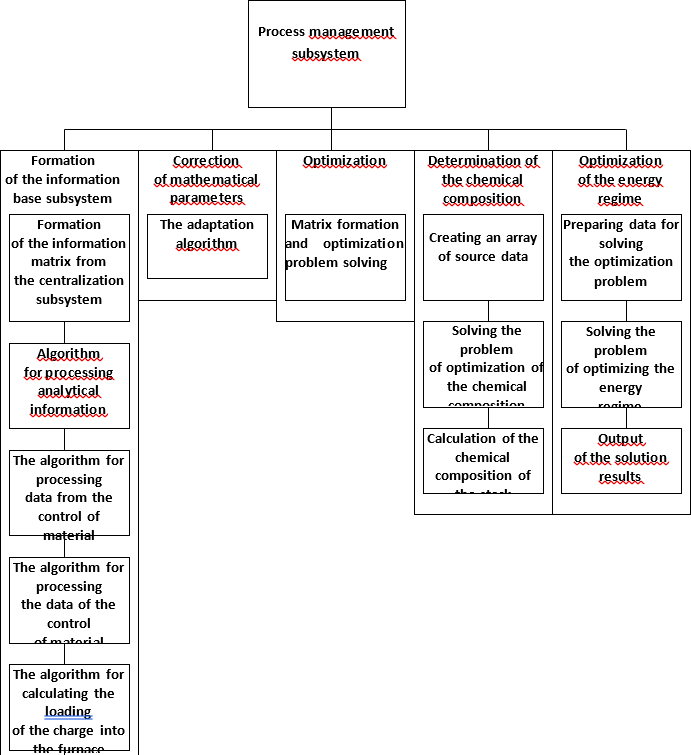
\includegraphics[width=0.6\textwidth]{assets/9}
	\caption*{Figure 2 - The block diagrams of these algorithms}
\end{figure}

\begin{noparindent}
Block 1. Enters the values of these variables
\(X_{ij},\ Y_{ij},\ a_{ij}\) into the machine.

Block 2. Checking the values of variables for validity.

Block 3. Checking for data sufficiency, in case of insufficiency, the
display unit 4 is triggered.

Block 5. The average values of the variables are found.

Block 6. The solution of equations is performed with the previous values
of the coefficients, the calculated \(\overline{y}\ \lbrack n\rbrack\)
data are compared with the experimental
\(\overline{y}\ \lbrack n,K\rbrack\).
\(\mathrm{\Delta}y\lbrack n,K\rbrack = \overline{y}\ \lbrack n\rbrack - \overline{y}\ \lbrack n,K\rbrack\)
is calculated.

Block 7. The comparison block. If the condition
\textbar∆y{[}n,K{]}\textbar≥∆ is fulfilled, block 8 is executed, which,
using block 9, leads to an adaptation, as a result of which new
coefficient values are obtained.

Block 10. Calculation of the optimal composition of the charge. At the
same time, we use the "Optimization" subroutine of block 11.
\end{noparindent}

The algorithm for adapting the mathematical model of the process of
mixing and melting copper concentrates is given below to the following
Equations 14-25:

\begin{equation}
f_{FeS}^{III} = \alpha_{FeS}^{II - III}G_{FeS}^{II} - K_{C}G_{FeS} - K_{mech}G_{FeS}^{III} - \alpha_{FeS}^{III - IV}\frac{\vartheta_{K}}{H_{sl}} = 0
\end{equation}

\begin{equation}
f_{Cu_{2}S}^{II} = \alpha_{Cu_{2}s}^{II - III}G_{Cu_{2}S}^{II} - K_{C}G_{Cu_{2}S} - G_{Cu_{2}S}G_{FeO} - K_{mech}G_{Cu_{2}S}^{III} - \alpha_{Cu_{2}S}^{III - IV}G_{Cu_{2}s}^{III}\frac{\vartheta_{K}}{H_{sl}} = 0
\end{equation}

\begin{equation}
f_{CaO}^{III} = \alpha_{CaO}^{II - III}G_{CaO} + \gamma_{CaO}^{K}G^{K} - \gamma_{CaO}G_{sl}^{m} = 0
\end{equation}

\begin{equation}
f_{SO_{2}}^{III} = \alpha_{SiO_{2}}^{II - III}G_{SiO_{2}}^{II} + \gamma_{SiO_{2}}^{K}G^{K} - \gamma_{SiO_{2}}G_{sl}^{m} = 0
\end{equation}

\begin{equation}
f_{Cao}^{II} = \alpha_{FeO}^{II - III}G_{FeO}^{II} + \gamma_{FeO}^{K}G^{K} - \gamma_{FeO}G_{sl}^{m} = 0
\end{equation}

\begin{equation}
G_{sl}^{II} = \beta_{1}G_{Cu_{2}S}^{III} + \beta_{2}G_{Cu_{2}O}^{III} + \beta_{3}G_{cp}^{III}
\end{equation}

\begin{equation}
С_{sl}^{II} = \gamma_{n}G_{Cu}^{III}
\end{equation}

\begin{equation}
F_{sl}^{II} = \rho_{sl}^{R} + k_{1}G_{SiO_{2}} + k_{2}G_{CaO} + k_{3}G_{FeO} + k_{4}t_{sl}
\end{equation}

\begin{equation}
f_{sl}^{II} = K_{э}\rho_{sl}^{R}I^{2} + G_{sl}^{K}С_{sl}^{к}t_{sl}^{K} - \alpha(t_{sl} - t_{m})ц_{0}С_{sl}F_{m} - \alpha(t_{sl} - t_{st})F_{st} - G_{sl}^{m}С_{sl}t_{sl} - \sum_{е}^{}\alpha_{е}^{III - IV}G_{e}C_{e}t_{sl}\frac{\vartheta_{к}}{Н_{sl}} = 0
\end{equation}

\begin{equation}
f_{Cu_{2}S}^{III} = \frac{\alpha_{Cu_{2}S}^{III - IV}G_{Cu_{2}S}^{III}}{H_{sl}}\vartheta_{k - \beta_{Cu_{2}S}G_{st}^{m}} = 0
\end{equation}

\begin{equation}
f_{FeS}^{II} = \frac{\alpha_{Cu_{2}S}^{III - IV}G_{Cu_{2}S}^{III}}{H_{sl}}\vartheta_{К} - \beta_{FeS}G_{st}^{вm} = 0
\end{equation}

\begin{equation}
f_{Fe}^{II} = (\sum_{l}^{}{\gamma_{l}G_{st}C_{е}})t_{sl} + \alpha(t_{sl} - t_{st})F_{st} - \lambda(\frac{t_{st} - t_{sl}}{\delta})h_{st}S_{n} - \frac{\lambda'}{\delta}(t_{st} - t_{n})F_{n} = 0
\end{equation}

The block diagram of the algorithm for optimal control of the energy
regime can be described as follows:

\begin{noparindent}
Blocks 1-6 . Collects, processes and generates mass data.

Blocks 7-20. The equations of the mathematical model of the electric
melting process are being implemented. The input of the blocks receives
information about the input parameters
\(\overline{G},\ \overline{H},\ \overline{U},\ \overline{H}\ Q_{c},\ G_{5_{p}}\)

Block 7. The equations of the material balance of the process are
implemented.

Block 8. The equations of the thermal process are calculated.

Block 9. Dependence of the resistivity of the charge and slag on the
input parameters determined on the basis of a study of factory slags.

Block 10. The equation of the dependence of the height of the slag bath
on the input parameters.

Block 11. Expression of the dependence of the slope depth on the input
parameters.

Blocks 12-16. The resistances of the equivalent electrical circuit of
the furnace are calculated as a function of the geometric parameters of
the specific resistances of the slag and charge and the phase voltage.

Block 17. The dependence of the phase power on the resistance of the
equivalent circuit and the phase voltage is realized.

Block 18. The dependence of the amount of matte on the input parameters
is determined.

Block 19. The dependences of the copper content in the dump slag on the
phase voltage and the electrode depth are realized.

Block 20. The specific consumption of electricity is determined,

Block 21. The adequacy of the mathematical model to the object is
checked. In case of inadequacy, he refers to the adaptation unit.

Block 22. The parameters of the mathematical model are adjusted
according to the well-known adaptation algorithm

Block 23. The optimal values of control actions are determined based on
the solution of the optimization problem.

Block 24. The optimization problem is solved using the Rosenbrock
method.

Block 25. The furnace operation is checked for accidents. In case of
failure to fulfill one of the conditions, a voltage reduction task is
issued.

Block 26. The actual voltage value is compared with the optimal one. In
the case of \(U_{real}\ \) going beyond the area \(|U -\)
\(U_{opt}|\varepsilon q\), a task is given to switch voltage stages in
one direction or the other.

Block 27. The actual conductivity is compared with the optimal one. In
case of going beyond the area
\(|q_{i} - q_{i\ opt}|\varepsilon q\)\emph{,} a task is given to bypass
the electrode in one direction or the other.

Block 28. The condition \(I \leq\) \(I_{con}\) is checked in the case of
a voltage increase task. If the condition is met, the voltage can be
increased.

Block 29. The position of the electrode holder is checked. If the
electrode holder is in the lowest position, a task is given to increase
the voltage. If not, the control is carried out by increasing the depth
of the electrode.

Block 30. It is checked whether the electrode holder is in the uppermost
position. If not, the electrode rises if a voltage reduction task is
issued.

Blocks 31-32. The magnitude of the control action (the number of voltage
stages) is determined and information is provided on which voltage stage
should be operated.

Blocks 33 - 34. An algorithm for direct control of electrode deepening
is implemented.
\end{noparindent}

The results of processing the data obtained during the two stages of the
tests are summarized in a table. The tests showed: the adequacy of
mathematical models of the process of electric melting of copper
concentrates and control tasks for a real object; the effectiveness of
the developed algorithms and programs for solving problems of optimal
calculation of the stack composition, distribution of material flows and
energy management

The used energy mode of electric melting for copper sulfide concentrates
made it possible to reduce the copper content in dump slags by 0.18\%
(absolute) and reduce copper losses with slags by 5\% (relative),
increase the copper content in matte by 0.97\% while reducing
electricity consumption by 1.8\%.

{\bfseries Conclusion.} Industrial tests and implementation of the electric
melting process control system were carried out in the electric furnace
department, pilot tests of the algorithm for controlling the process of
electric melting of copper concentrates in industrial conditions were
carried out.

The tests were carried out in order to: clarify the coefficients of the
mathematical model; verify the adequacy of the mathematical model of
control tasks; adjust algorithms and programs in industrial conditions;
verify the effectiveness of the developed algorithms and programs. The
tests were carried out in accordance with the program and methodology.

The results of theoretical and experimental studies on the control
system for the process of electric melting of copper sulfide
concentrates are the basis for the design solutions of the Institute of
Information and Computational Technologies CS MSHE RK.

\emph{{\bfseries Financing.} Research were carried out within the framework
of the Grant Financing Project No. AP19679153 ``Research and development
of method and technologies for creating composite structures with
built-in photonic sensors PSBC (Photonic Smart Bragg Composites)''
Institute of Information and Computational Technologies of the Science
Committee of the Ministry of Science and Higher Education of the
Republic of Kazakhstan.}

\begin{center}
{\bfseries References}
\end{center}

\begin{noparindent}
1.Istadi I., Bindar Y. Improved cooler design of~electric~arc furnace
refractory in mining industry using thermal analysis modeling and
simulation.//Applied Thermal Engineering.- 2014.- Vol.73, Iss.1.-
P.1129-1140.

https://doi.org/10.1016/j.applthermaleng.2014.08.070

2.Imanbekova U., Hotra O., Koshimbayev S., Optimal control of copper
concentrate blending and melting based on intelligent systems.// Journal
Przegląd Elektrotechniczny.2016.-Vol.8.- P.125-128.
doi:10.15199/48.2016.08.34

3.Malfliet A., Lotfian S., Scheunis L., Petkov V., Pandelaers L., Jones
P.T., Blanpain B. Degradation mechanisms and use of refractory linings
in copper production processes // Journal of the European Ceramic
Society. A critical review.- 2014.- Vol.34, Iss.3. - P. 849-876.
https://doi.org/10.1016/j.jeurceramsoc.2013.10.005

4.Cheng P., Herreros P., Lalpuria M., Grossmann I. Optimal scheduling of
copper concentrate operations under uncertainty.//Computers \& Chemical
Engineering.-2020.- Vol.140, 106919.

doi.org/10.1016/j.compchemeng.2020.106919

5.Guimarães F.Y., Santos I.D., Dutra J.B. Direct recovery of~copper~from
printed circuit boards (PCBs) powder concentrate by a simultaneous
electroleaching--electrodeposition~process.//
Hydrometallurgy.-2014.-Vol. 149.- P. 63-70.

https://doi.org/10.1016/j.hydromet.2014.06.005

6.Zhai Q.,Runqing Lui. Simultaneous recovery of arsenic and copper from
copper smelting slag by flotation: Redistribution behavior and toxicity
investigation. Journal of Cleaner Production. -2023.-Vol. 425, 138811

https://doi.org/10.1016/j.jclepro.2023.138811

7.Imanbekova U., Hotra O., Koshimbayev S. K., Popiel P., Tanas J.
Optimal control of blending and melting of copper concentrates.//
Proceedings of SPIE-The International Society for Optical Engineering
.-2015, 966246. DOI:10.1117/12.2205446

8.Rubanenko O. O., Komar V. O., Petrushenko O. Y., Smolarz A., Smailova
S., Imanbekova U., Determinition of similatiry criteria in optimization
tasks by means of neuro-fuzzy modelling. //Journal Przegląd
Elektrotechniczny.-2017.-Vol. 1(3).- P.95-98. DOI:10.15199/48.2017.03.22

9.Hotra O.Z., Koshimbayev S.K., Imanbekova U.N. Modelling in Matlab
using fuzzy logic for improving the economic factors of melting of
copper concentrate charge.// Actual problems of
economics.-2014.-Vol.11.-P. 380-387.

10.Da-wei~Wang,~Yan-jie~Liang. Comprehensive recovery of zinc, iron and
copper from copper slag by co-roasting with SO2--O2./ Journal of
Materials Research and Technology.-2022.- Vol.19.-P.2546-2555.

https://doi.org/10.1016/j.jmrt.2022.05.177
\end{noparindent}

\emph{{\bfseries Information about authors}}

\begin{noparindent}
U. Imanbekova -PhD, Associate Professor, Almaty University of Power
Engineering and Telecommunications named after G.Daukeyev, Almaty,
Kazakhstan, e-mail: uli.08@mail.ru;

A.Kalizhanova- Professor, Institute of Information and Computational
Technologies CS MSHE RK, Almaty, Kazakhstan, Almaty University of Power
Engineering and Telecommunications named after G.Daukeyev, Almaty,
Kazakhstan, e-mail: kalizhanova.aliya@gmail.com;

A.Kozbakova - PhD, Institute of Information and Computational
Technologies CS MSHE RK, Almaty,Kazakhstan, Almaty Technological
University, Almaty, Kazakhstan, e-mail: ainur79@mail.ru;

A.Imanbekova- Senior Lecturer, M. H. Dulati Taraz Regional University,
Taraz, Kazakhstan, e-mail: aleka.12@mail.ru;

A.Utegenova -PhD, Institute of Information and Computational
Technologies CS MSHE RK, Almaty, Kazakhstan, Almaty University of Power
Engineering and Telecommunications named after G.Daukeyev, Almaty,
Kazakhstan, e-mail: an.utegenova@aues.kz
\end{noparindent}

\emph{{\bfseries Сведения об авторах}}

\begin{noparindent}
Иманбекова У. -PhD., ассоциированный профессор, Алматинский университет
энергетики и связи им. Г. Даукеева, Алматы, Казахстан, e-mail:
uli.08@mail.ru;

Калижанова А. - к.ф.-м.н., профессор, Институт информационных и
вычислительных технологий КН МНВО РК. Алматинский университет энергетики
и связи им. Г. Даукеева, Алматы, Казахстан, e-mail:

kalizhanova.aliya@gmail.com;

Козбакова А.- PhD, Институт информационных и вычислительных технологий
КН МНВО РК, Алматинский технологический университет, Алматы, Казахстан,
e-mail: ainur79@mail.ru;

Иманбекова А.- старший преподаватель, Таразский региональный университет
им.М. Х. Дулати, Тараз, Казахстан, e-mail: aleka.12@mail.ru;

Утегенова А.-PhD Институт информационных и вычислительных технологий КН
МНВО РК, Алматинский университет энергетики и связи им. Г. Даукеева,
Алматы, Казахстан, e-mail: an.utegenova@aues.kz
\end{noparindent}
